% !TEX program = xelatex
\documentclass{beamer}
\usetheme{Antibes}
\usepackage{mdframed}
\usepackage{hyperref}
\usepackage{mciteplus}
\usepackage{graphicx}
\usepackage{float}
\usepackage{caption, subcaption}
\usepackage{tabularx}
\usepackage{tikz}
\usepackage{fontspec}
\usepackage[super]{nth}

\setbeamertemplate{footline}[frame number]
\usefonttheme{serif}
\setmainfont{Times New Roman}
\setsansfont{DejaVu Sans}



\definecolor{myblue}{RGB}{91,155,213}
\definecolor{myyellow}{RGB}{237,125,49}
\newcommand{\circled[2]}{
	\tikzset{mystyle/.style={circle,#1,minimum size=10,inner sep=0pt}}
	\tikz[baseline=-3pt]
	{
		\node[mystyle] (char.center) {\vphantom{WAH1g}#2};
	}
}

\title{BadUSB-C: Revisiting BadUSB with Type-C}
\author{\textit{Hongyi Lu}, Yechang Wu, Shuqing Li, You Lin, Chaozu Zhang Fengwei Zhang}
\institute{Southern University of Science and Technology}
\date{\today}
\setcounter{tocdepth}{1}
\begin{document}
\begin{frame}
	\vfill
	\titlepage
	\vfill
\end{frame}
\begin{frame}{Outline}
	\tableofcontents
\end{frame}
\section{Background}
\subsection{USB Protocol}
\begin{frame}{The Ubiquitous Peripheral}
	\begin{figure}[htbp]
		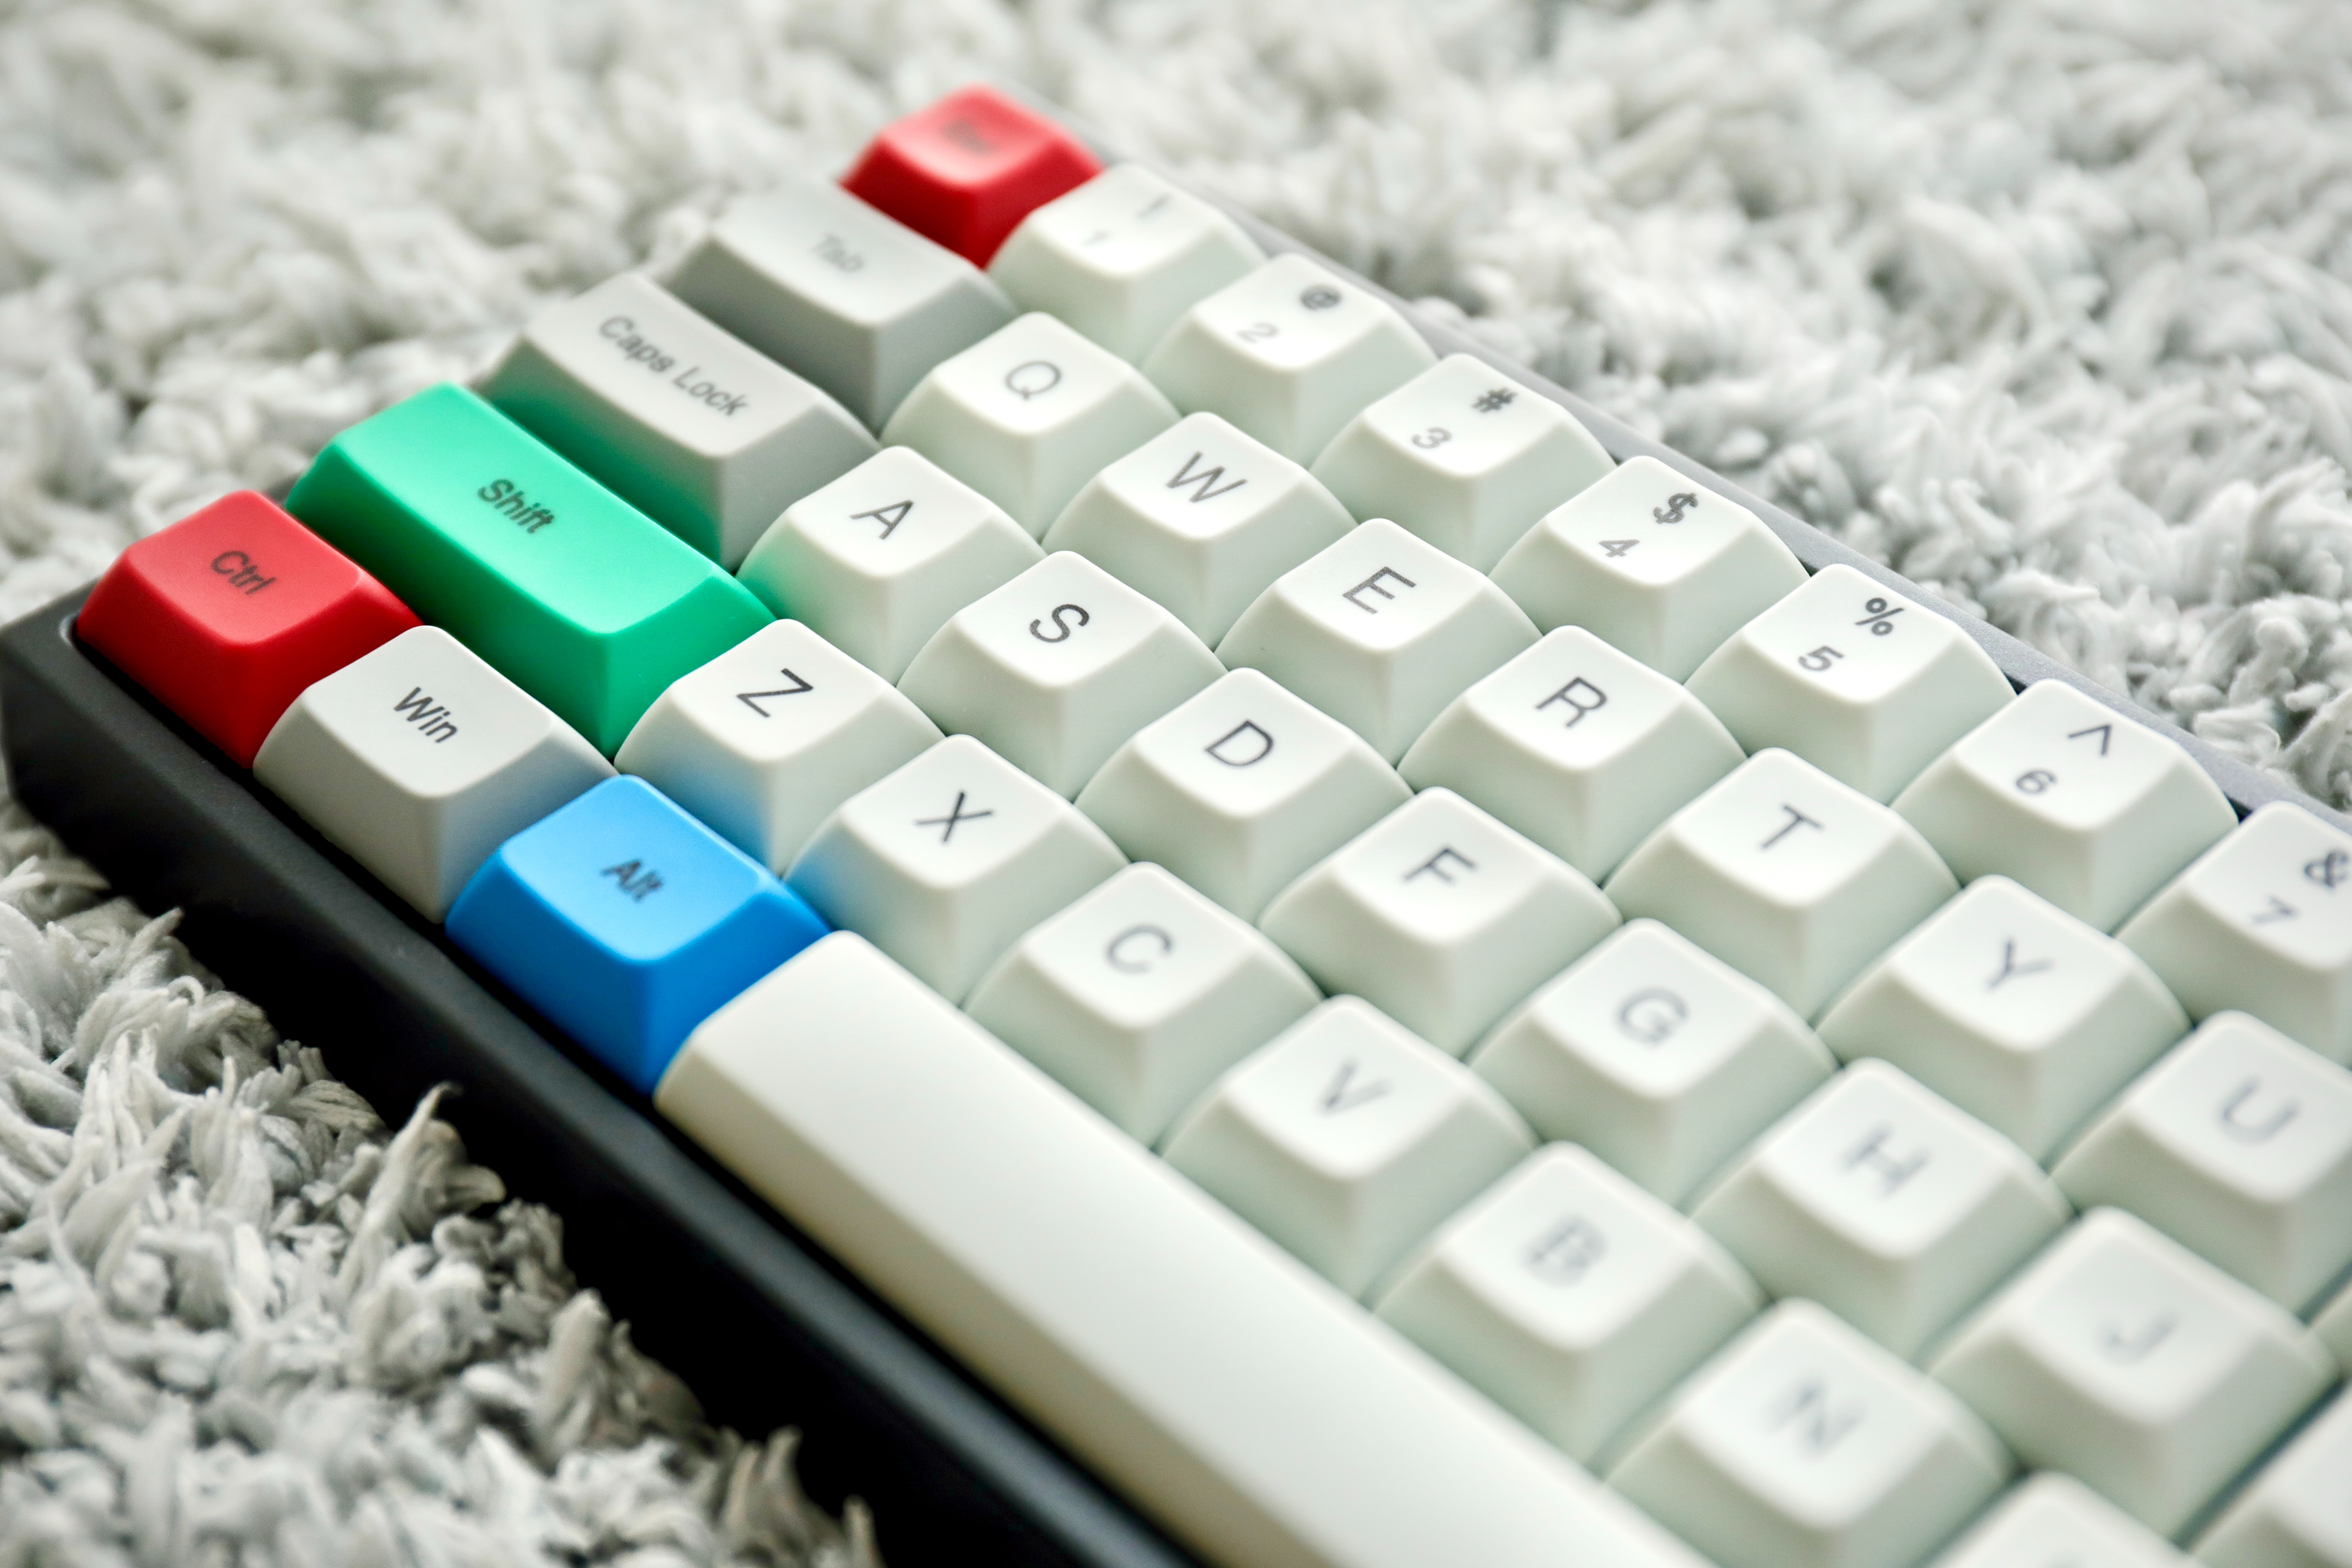
\includegraphics[width=.7\textwidth]{Figs/keyboard.jpg}
		\caption*{HIDs}
	\end{figure}
\end{frame}
\begin{frame}{The Ubiquitous Peripheral}
	\begin{figure}[htbp]
		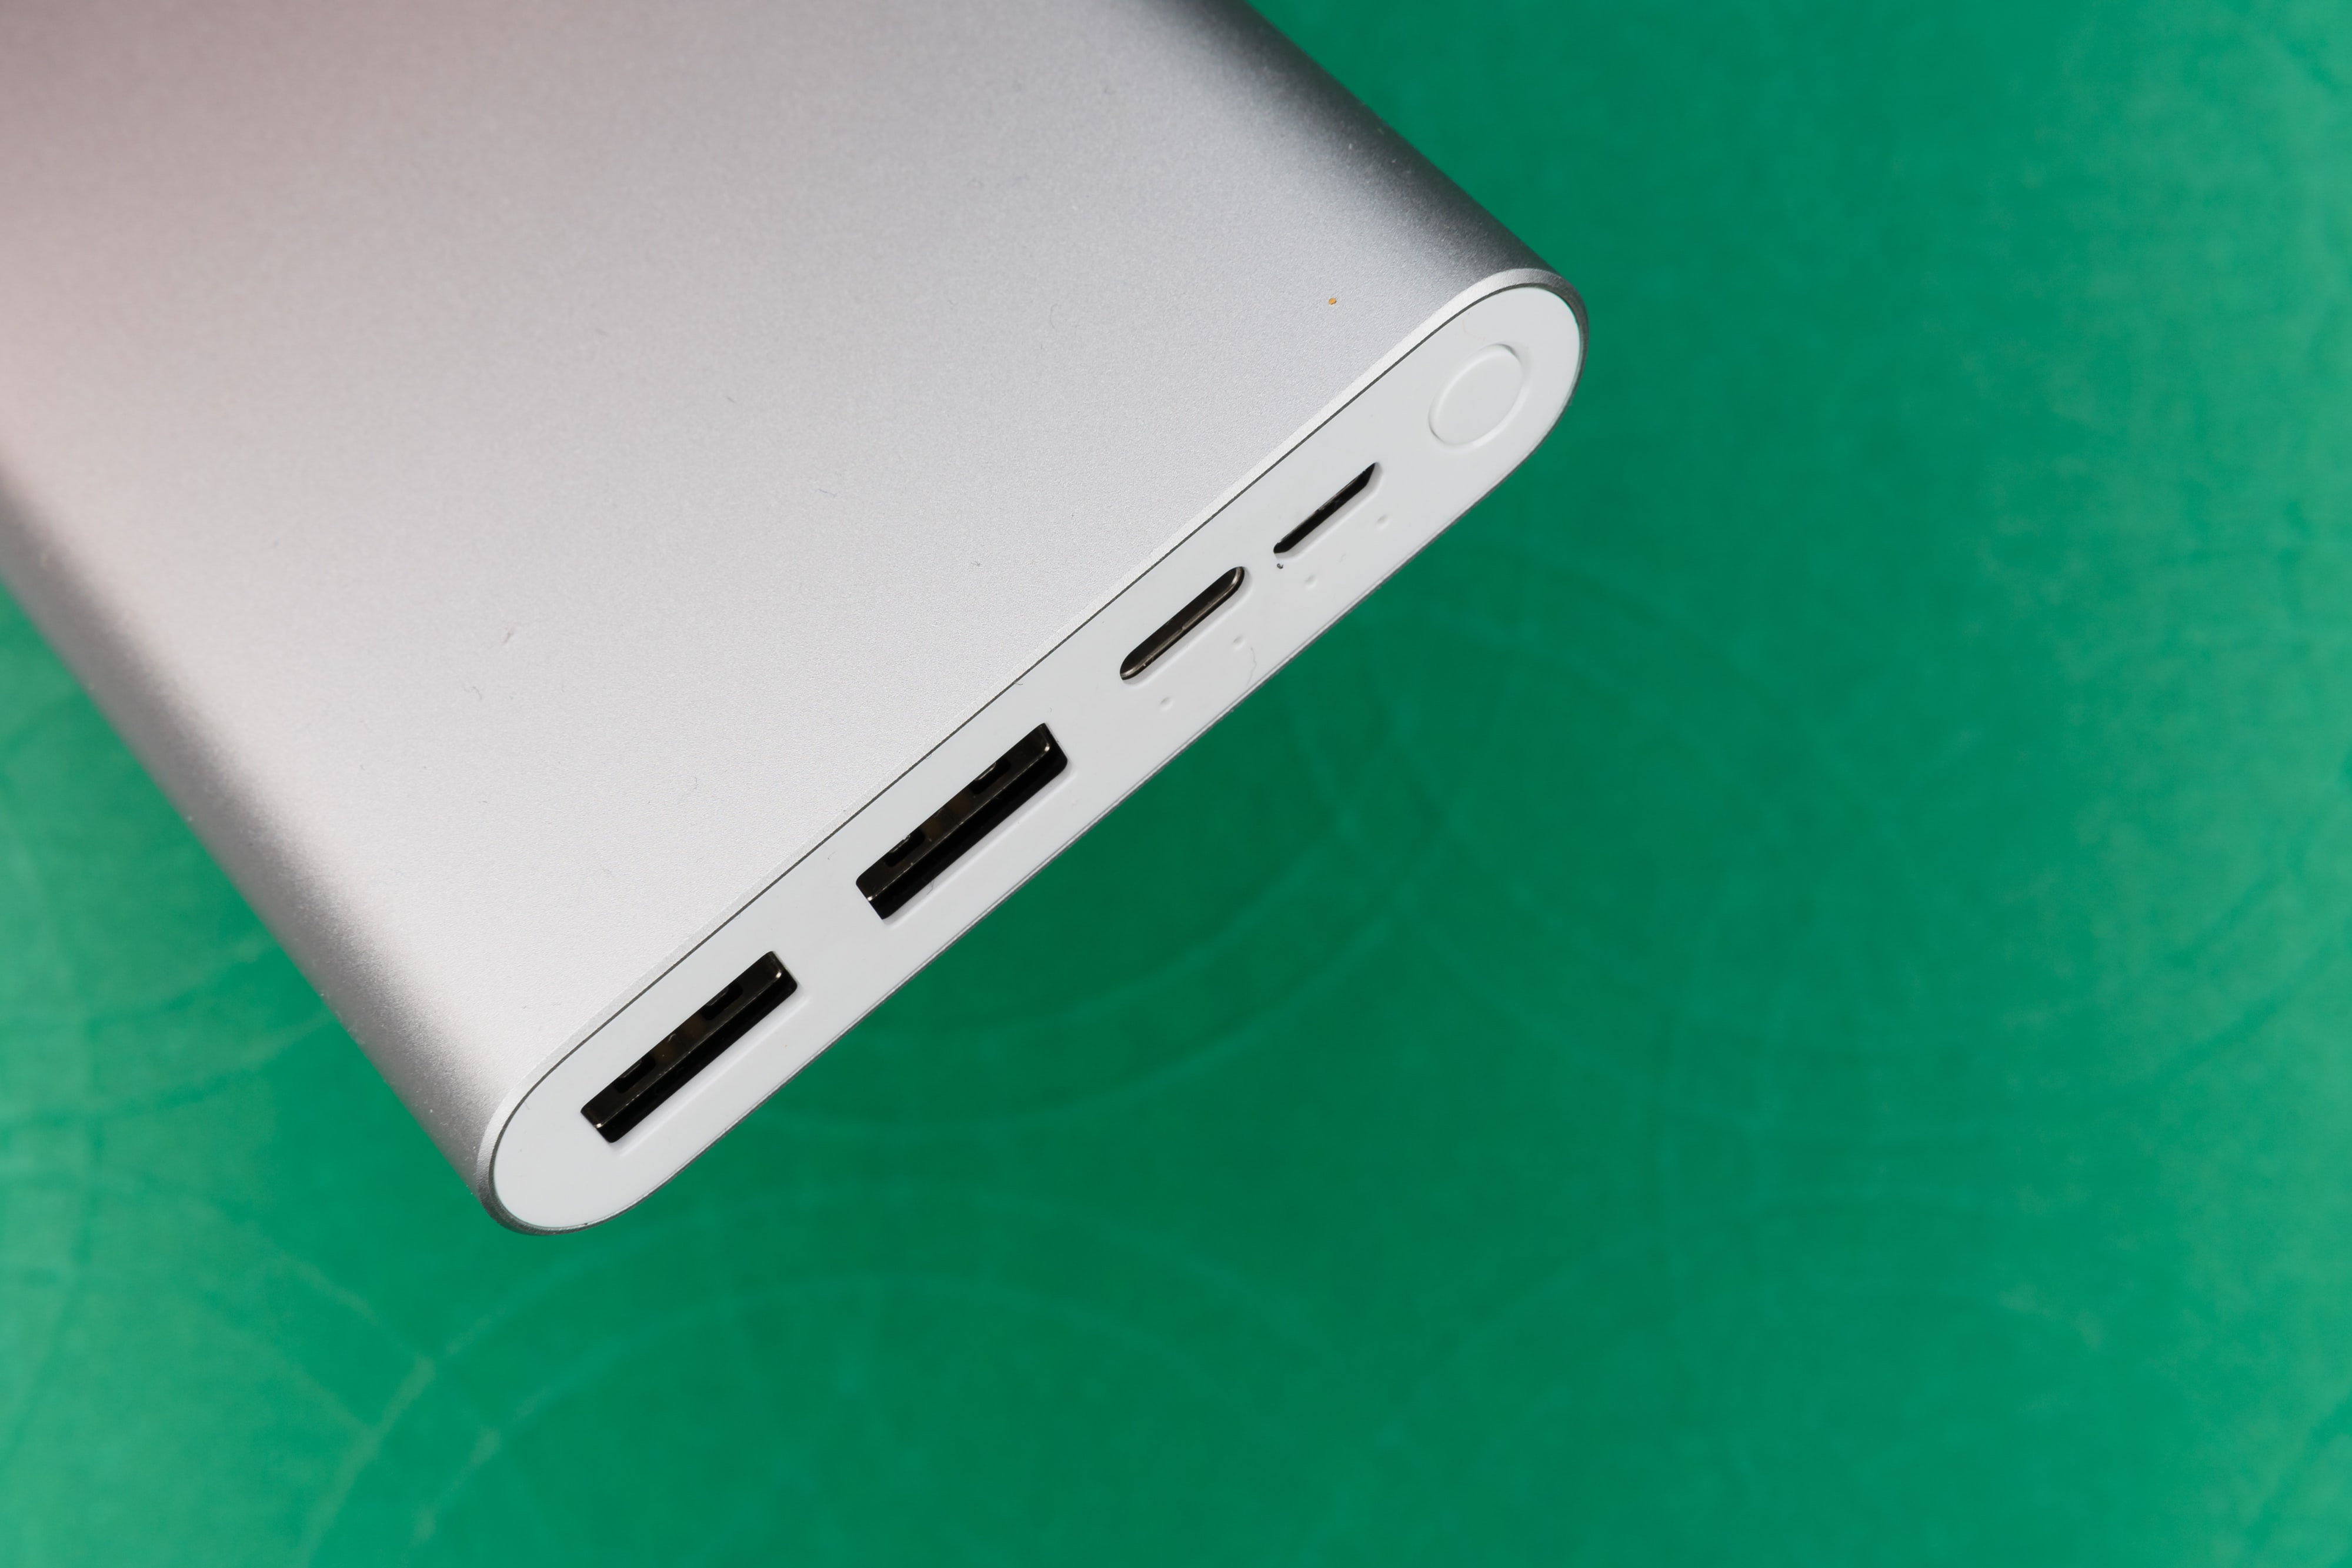
\includegraphics[width=.7\textwidth]{Figs/powerbank.jpg}
		\caption*{Charging}
	\end{figure}
\end{frame}
\begin{frame}{The Ubiquitous Peripheral}
	\begin{figure}[htbp]
		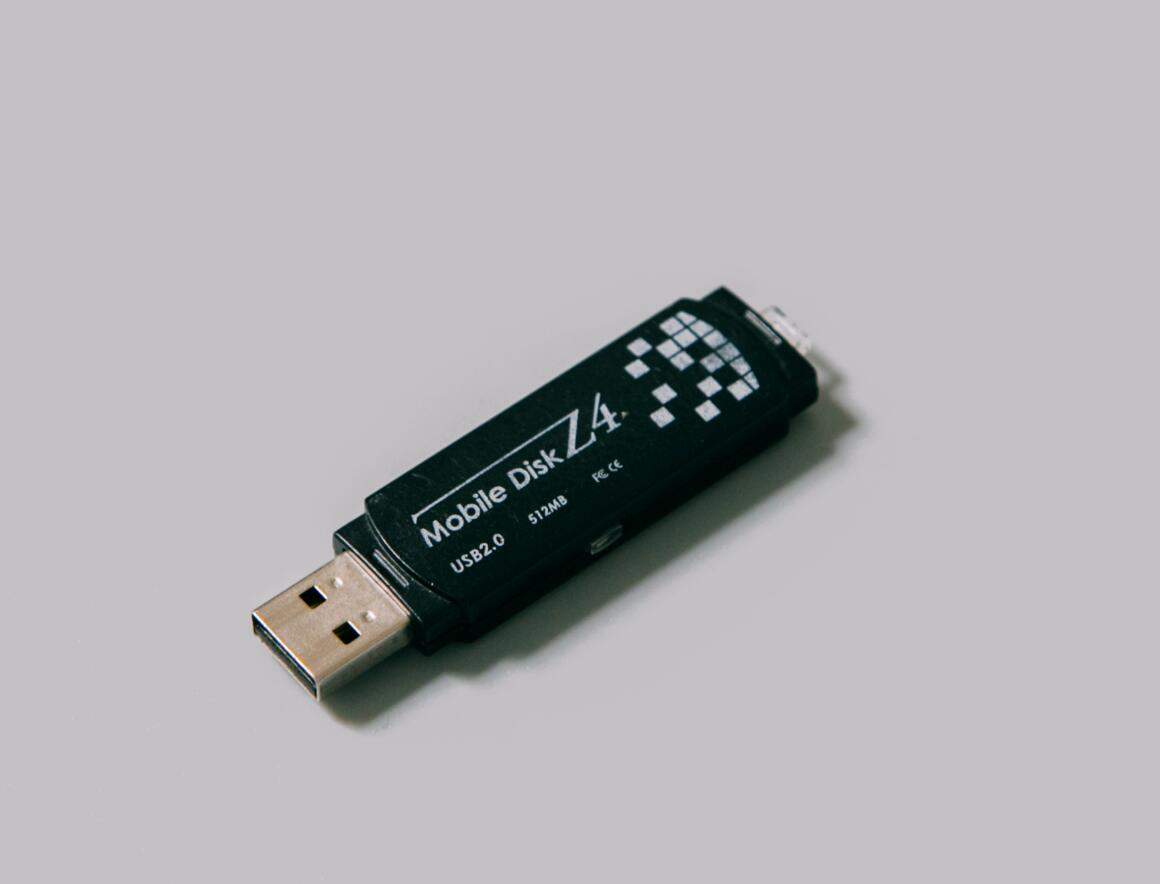
\includegraphics[width=.7\textwidth]{Figs/flashdrive.jpg}
		\caption*{Data Transfer}
	\end{figure}
\end{frame}
\subsection{Type-C Connector}
\begin{frame}{All in One With Type-C}
\begin{figure}[htbp]
	\includegraphics<1>[width=.8\textwidth]{Figs/messy_cables.png}
	\includegraphics<2>[width=.8\textwidth]{Figs/usbc_top.jpg}
\end{figure}
\end{frame}
\subsection{USB Vulnerabilities}
\begin{frame}{With Great Power Comes Great Responsibility}
	\begin{table}
		\begin{tabular}{c|l|c|c}
			\textbf{Year} & \textbf{Version} & \textbf{Peripherals} & \textbf{Attacks} \\
			1996 & USB 1.x~\cite{usb10,usb11} & Keyboard, Mouse... & BadUSB~\cite{badusb}... \\
			2000 & USB 2.0~\cite{usb20} & Flash Drive, CD Driver... & / \\
			2008 & USB 3.0~\cite{usb30} & /  & / \\
			2013 & USB 3.1~\cite{usb31} &  DisplayPort, ThunderBolt...  & \textbf{BadUSB-C} \\
			2017 & USB 3.2~\cite{usb32} & /  & / \\
		\end{tabular}
		\linebreak
		\caption*{USB Protocol Timeline.}
	\end{table}
\end{frame}
\subsection{Motivations}
\begin{frame}{Traditional BadUSB}
	\begin{figure}[htbp]
		\includegraphics<1>[width=.8\textwidth]{Figs/BadUSB_1.png}
		\includegraphics<2>[width=.8\textwidth]{Figs/BadUSB_2.png}
		\includegraphics<3>[width=.8\textwidth]{Figs/BadUSB_3.png}
		\caption*{Traditional BadUSB Attack.}
	\end{figure}
\end{frame}
\begin{frame}{BadUSB Limitations}
	There are some limitations of the traditional BadUSB attack.
	\begin{itemize}
		\item Cannot perform attack precisely.
		\item Cannot interact with GUI.
		\item Require host network usage.
	\end{itemize}
\end{frame}
\section{Design \& Prototype}
\subsection{Design}
\begin{frame}{Overview}
	\begin{figure}[htbp]
		\centering
		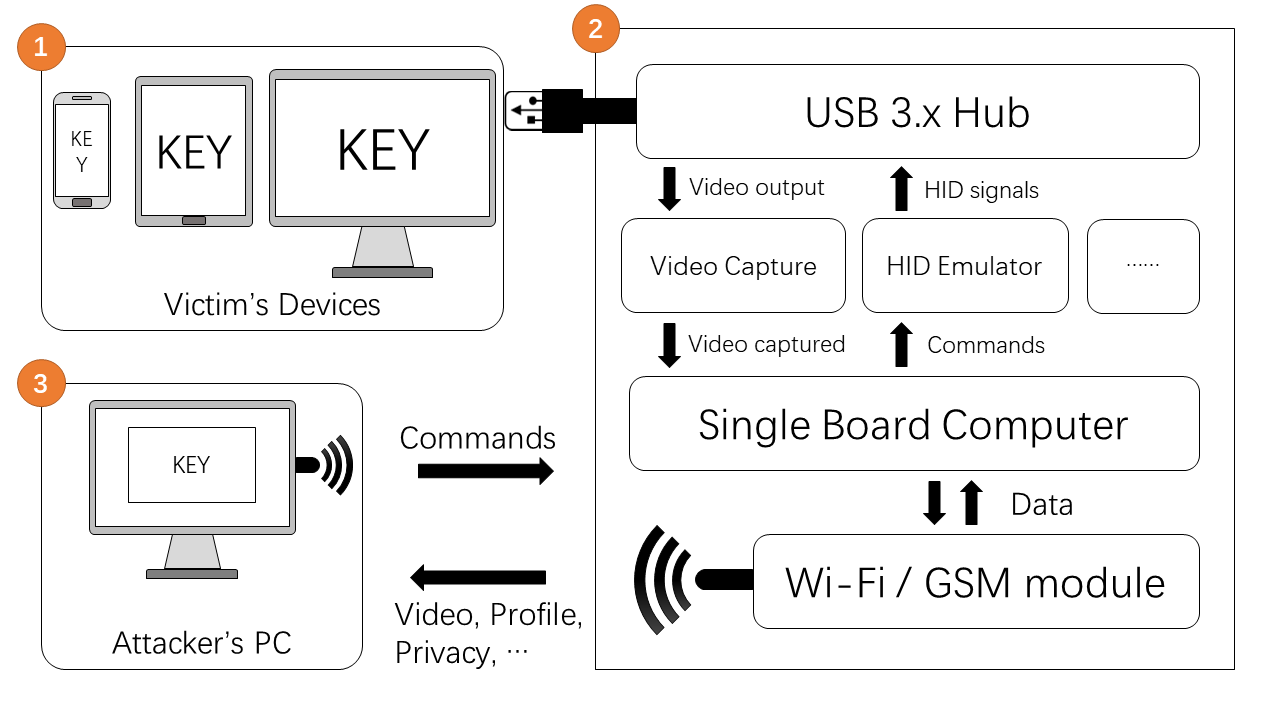
\includegraphics[width=.8\textwidth]{Figs/attack_model.png}
		\begin{tabular}{ll}
			\circled[text=white,fill=myyellow]{\footnotesize{1}} Victim's Devices    &\circled[text=white,fill=myyellow]{\footnotesize{2}}~BadUSB-C\\
			\circled[text=white,fill=myyellow]{\footnotesize{3}} Attacker's Remote PC
		\end{tabular}
	\end{figure}
\end{frame}
\begin{frame}{Video Path}
	\begin{figure}[htbp]
		\centering
		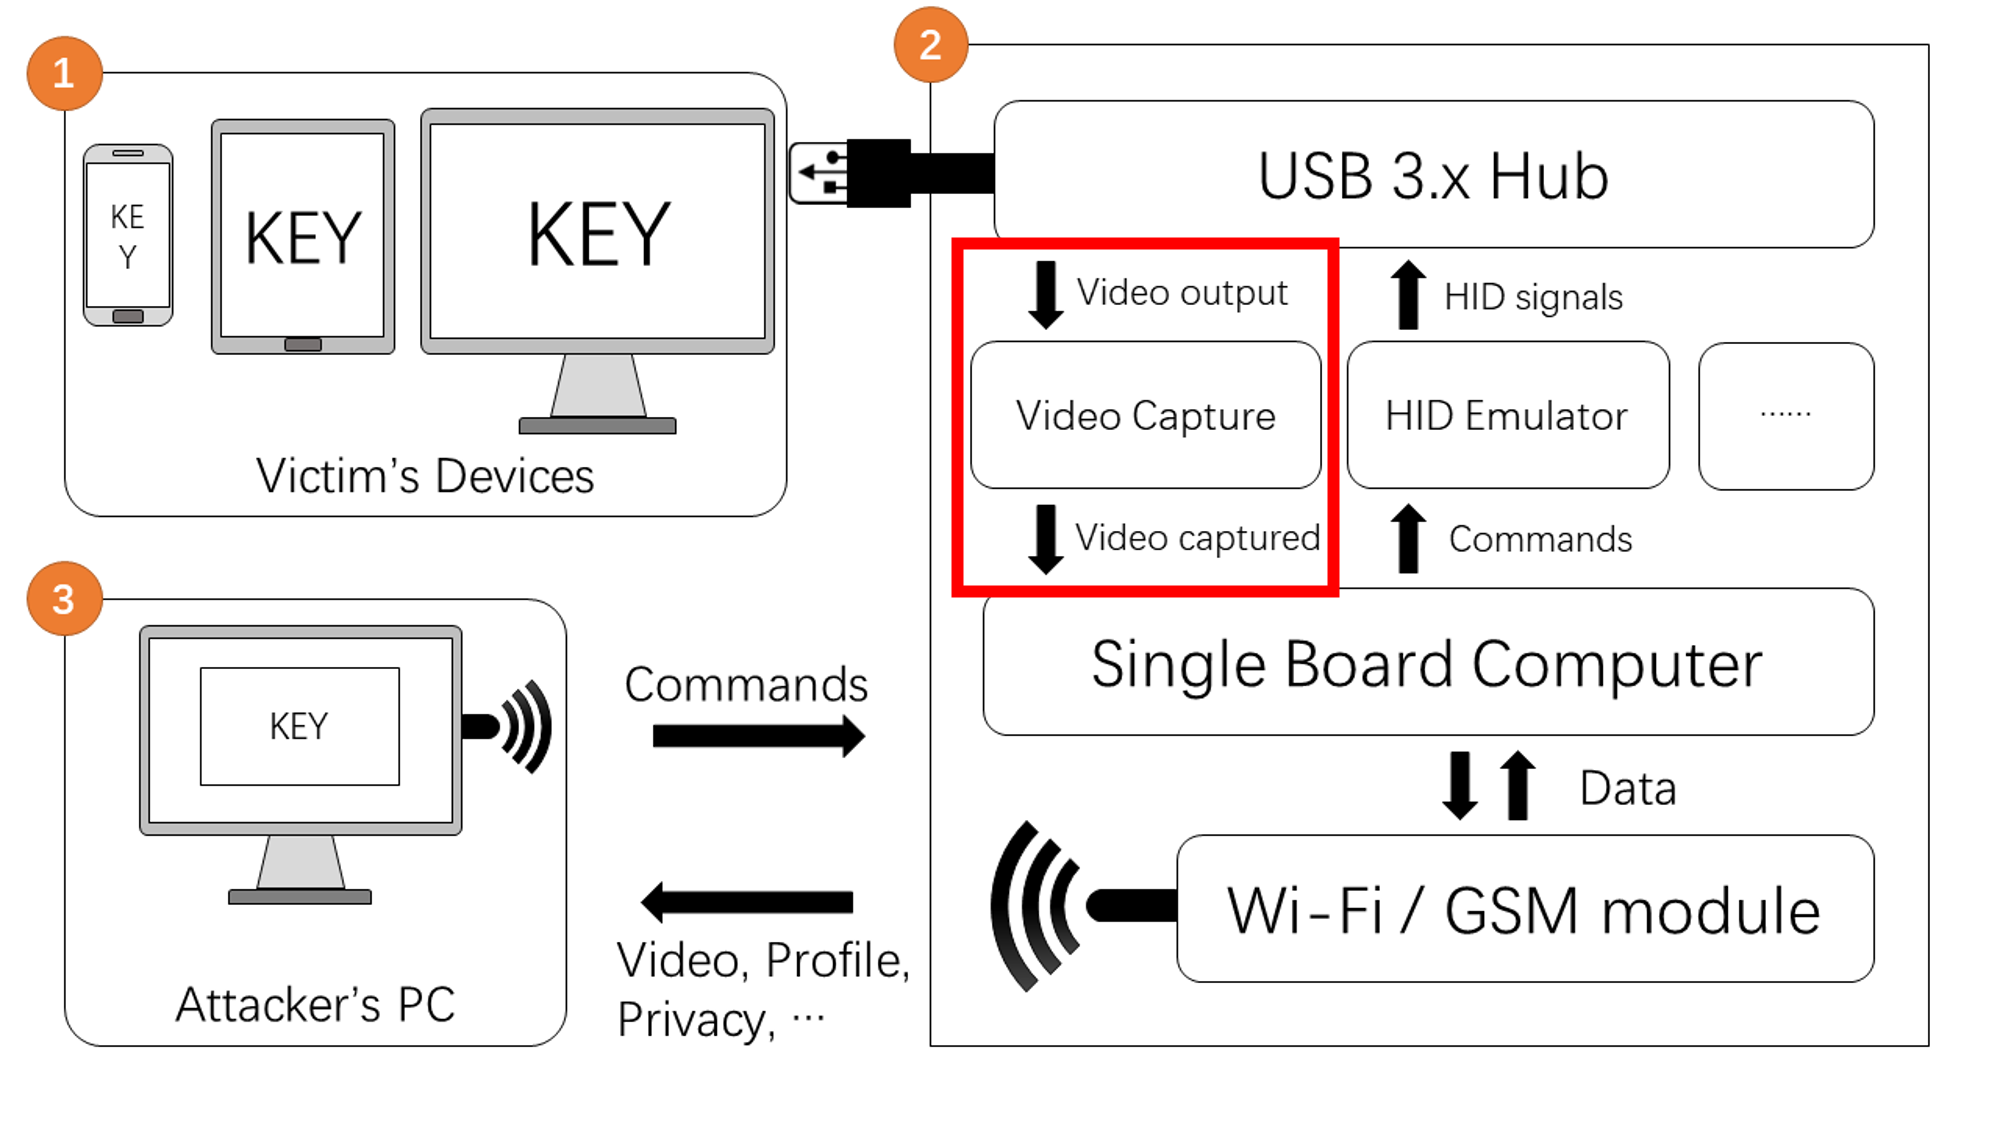
\includegraphics[width=.8\textwidth]{Figs/video_path.png}
		\begin{tabular}{ll}
			\circled[text=white,fill=myyellow]{\footnotesize{1}} Victim's Devices    &\circled[text=white,fill=myyellow]{\footnotesize{2}}~BadUSB-C\\
			\circled[text=white,fill=myyellow]{\footnotesize{3}} Attacker's Remote PC
		\end{tabular}
	\end{figure}
\end{frame}
\begin{frame}{HID Path}
	\begin{figure}[htbp]
		\centering
		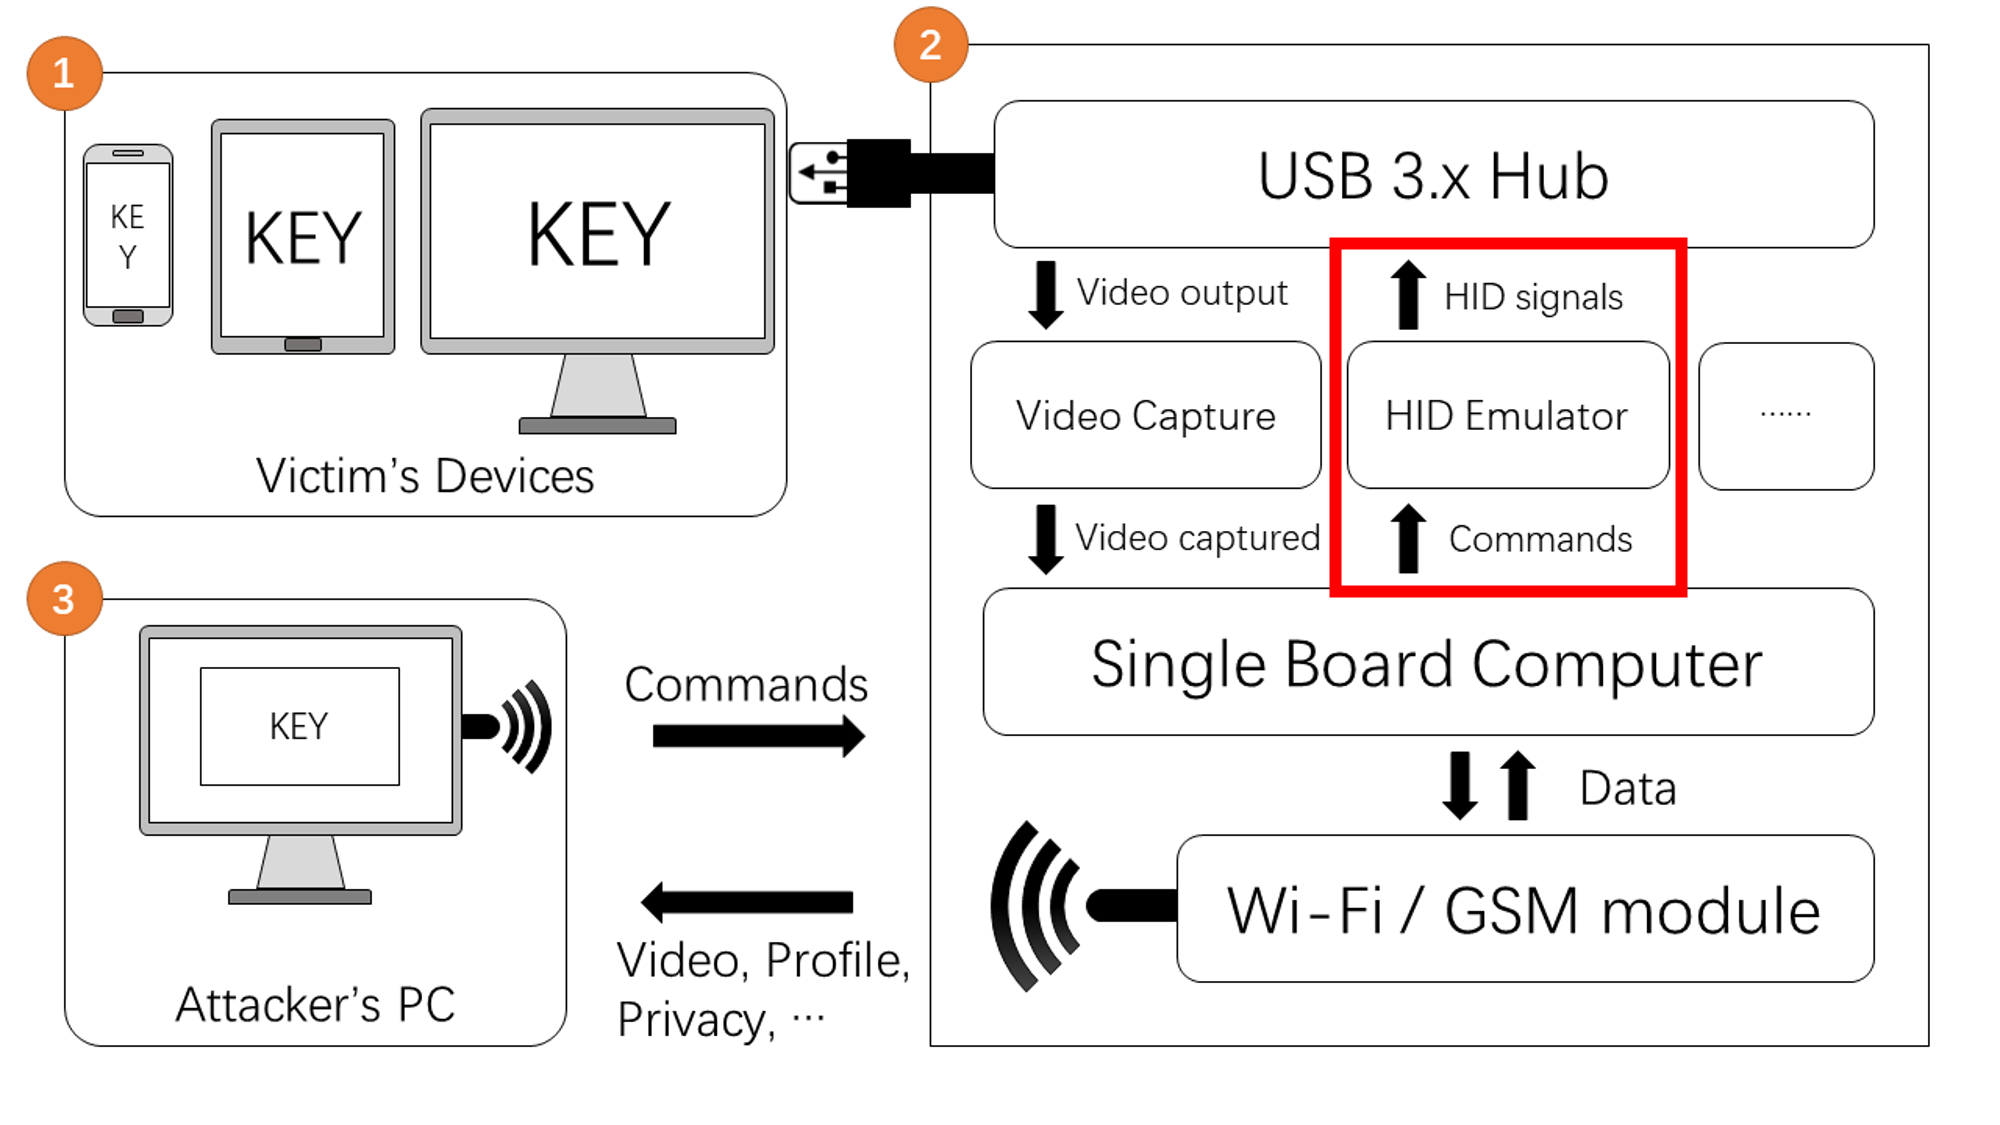
\includegraphics[width=.8\textwidth]{Figs/hid_path.png}
		\begin{tabular}{ll}
			\circled[text=white,fill=myyellow]{\footnotesize{1}} Victim's Devices    &\circled[text=white,fill=myyellow]{\footnotesize{2}}~BadUSB-C\\
			\circled[text=white,fill=myyellow]{\footnotesize{3}} Attacker's Remote PC
		\end{tabular}
	\end{figure}
\end{frame}
\begin{frame}{Individual WiFi/GSM}
	\begin{figure}[htbp]
		\centering
		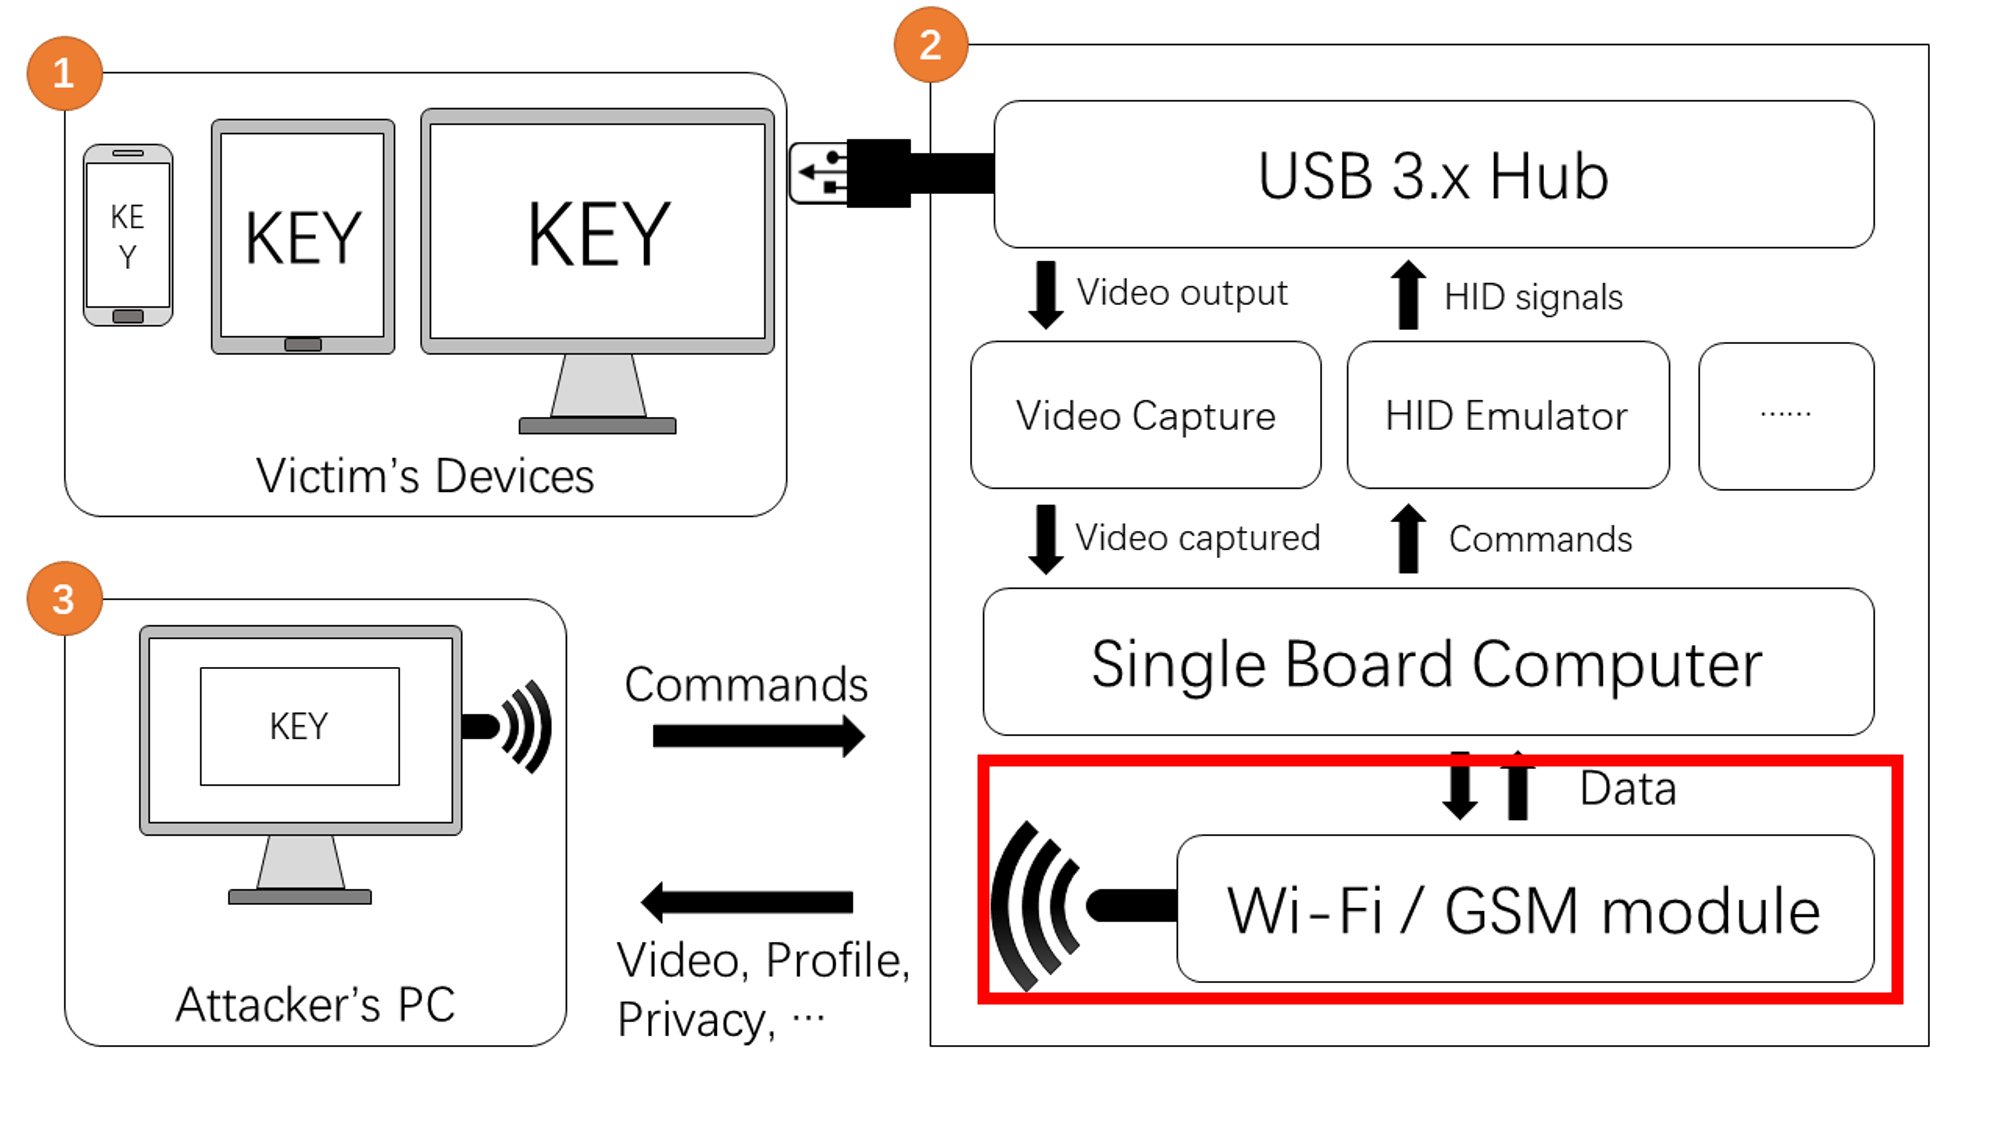
\includegraphics[width=.8\textwidth]{Figs/individual_wifi.png}
		\begin{tabular}{ll}
			\circled[text=white,fill=myyellow]{\footnotesize{1}} Victim's Devices    &\circled[text=white,fill=myyellow]{\footnotesize{2}}~BadUSB-C\\
			\circled[text=white,fill=myyellow]{\footnotesize{3}} Attacker's Remote PC
		\end{tabular}
	\end{figure}
\end{frame}
\subsection{Prototype}
\begin{frame}{Prototype}
	\centering
	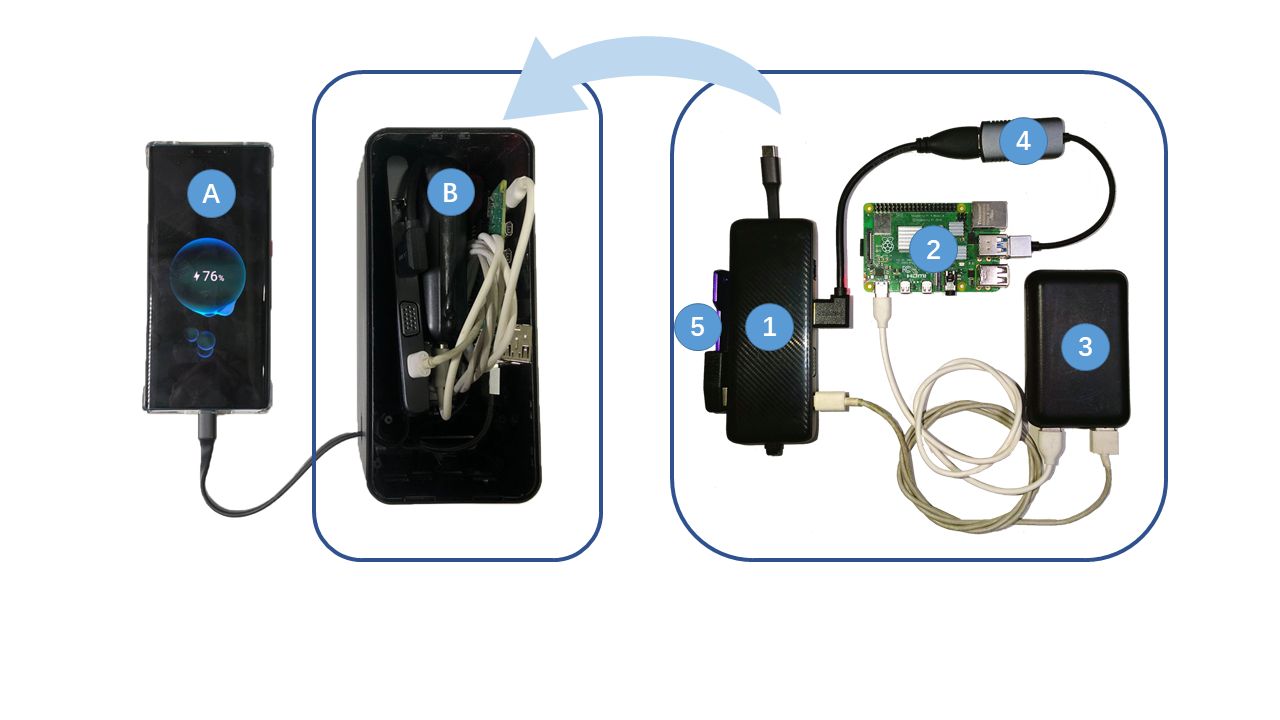
\includegraphics[width=.8\textwidth]{Figs/armory_all.png}
		\begin{tabular}{ll}
		\circled[text=white,fill=myblue]{\scriptsize{A}} Victim's Device    &\circled[text=white,fill=myblue]{\scriptsize{B}}~BadUSB-C\\
		\circled[text=white,fill=myblue]{\footnotesize{1}} USB 3.x Hub        &\circled[text=white,fill=myblue]{\footnotesize{2}} Raspberry Pi 4B\\
		\circled[text=white,fill=myblue]{\footnotesize{3}} Auxiliary Power Bank &\circled[text=white,fill=myblue]{\footnotesize{4}} Video Capture\\
		\circled[text=white,fill=myblue]{\footnotesize{5}} ATMEGAA32U4 Board
	\end{tabular}
\end{frame}
\section{Case Study}
\subsection{Background}
\begin{frame}{Sharing Powerbank}
	\begin{figure}[htbp]
		\centering
		\begin{minipage}[t]{0.4\textwidth}
			\centering
			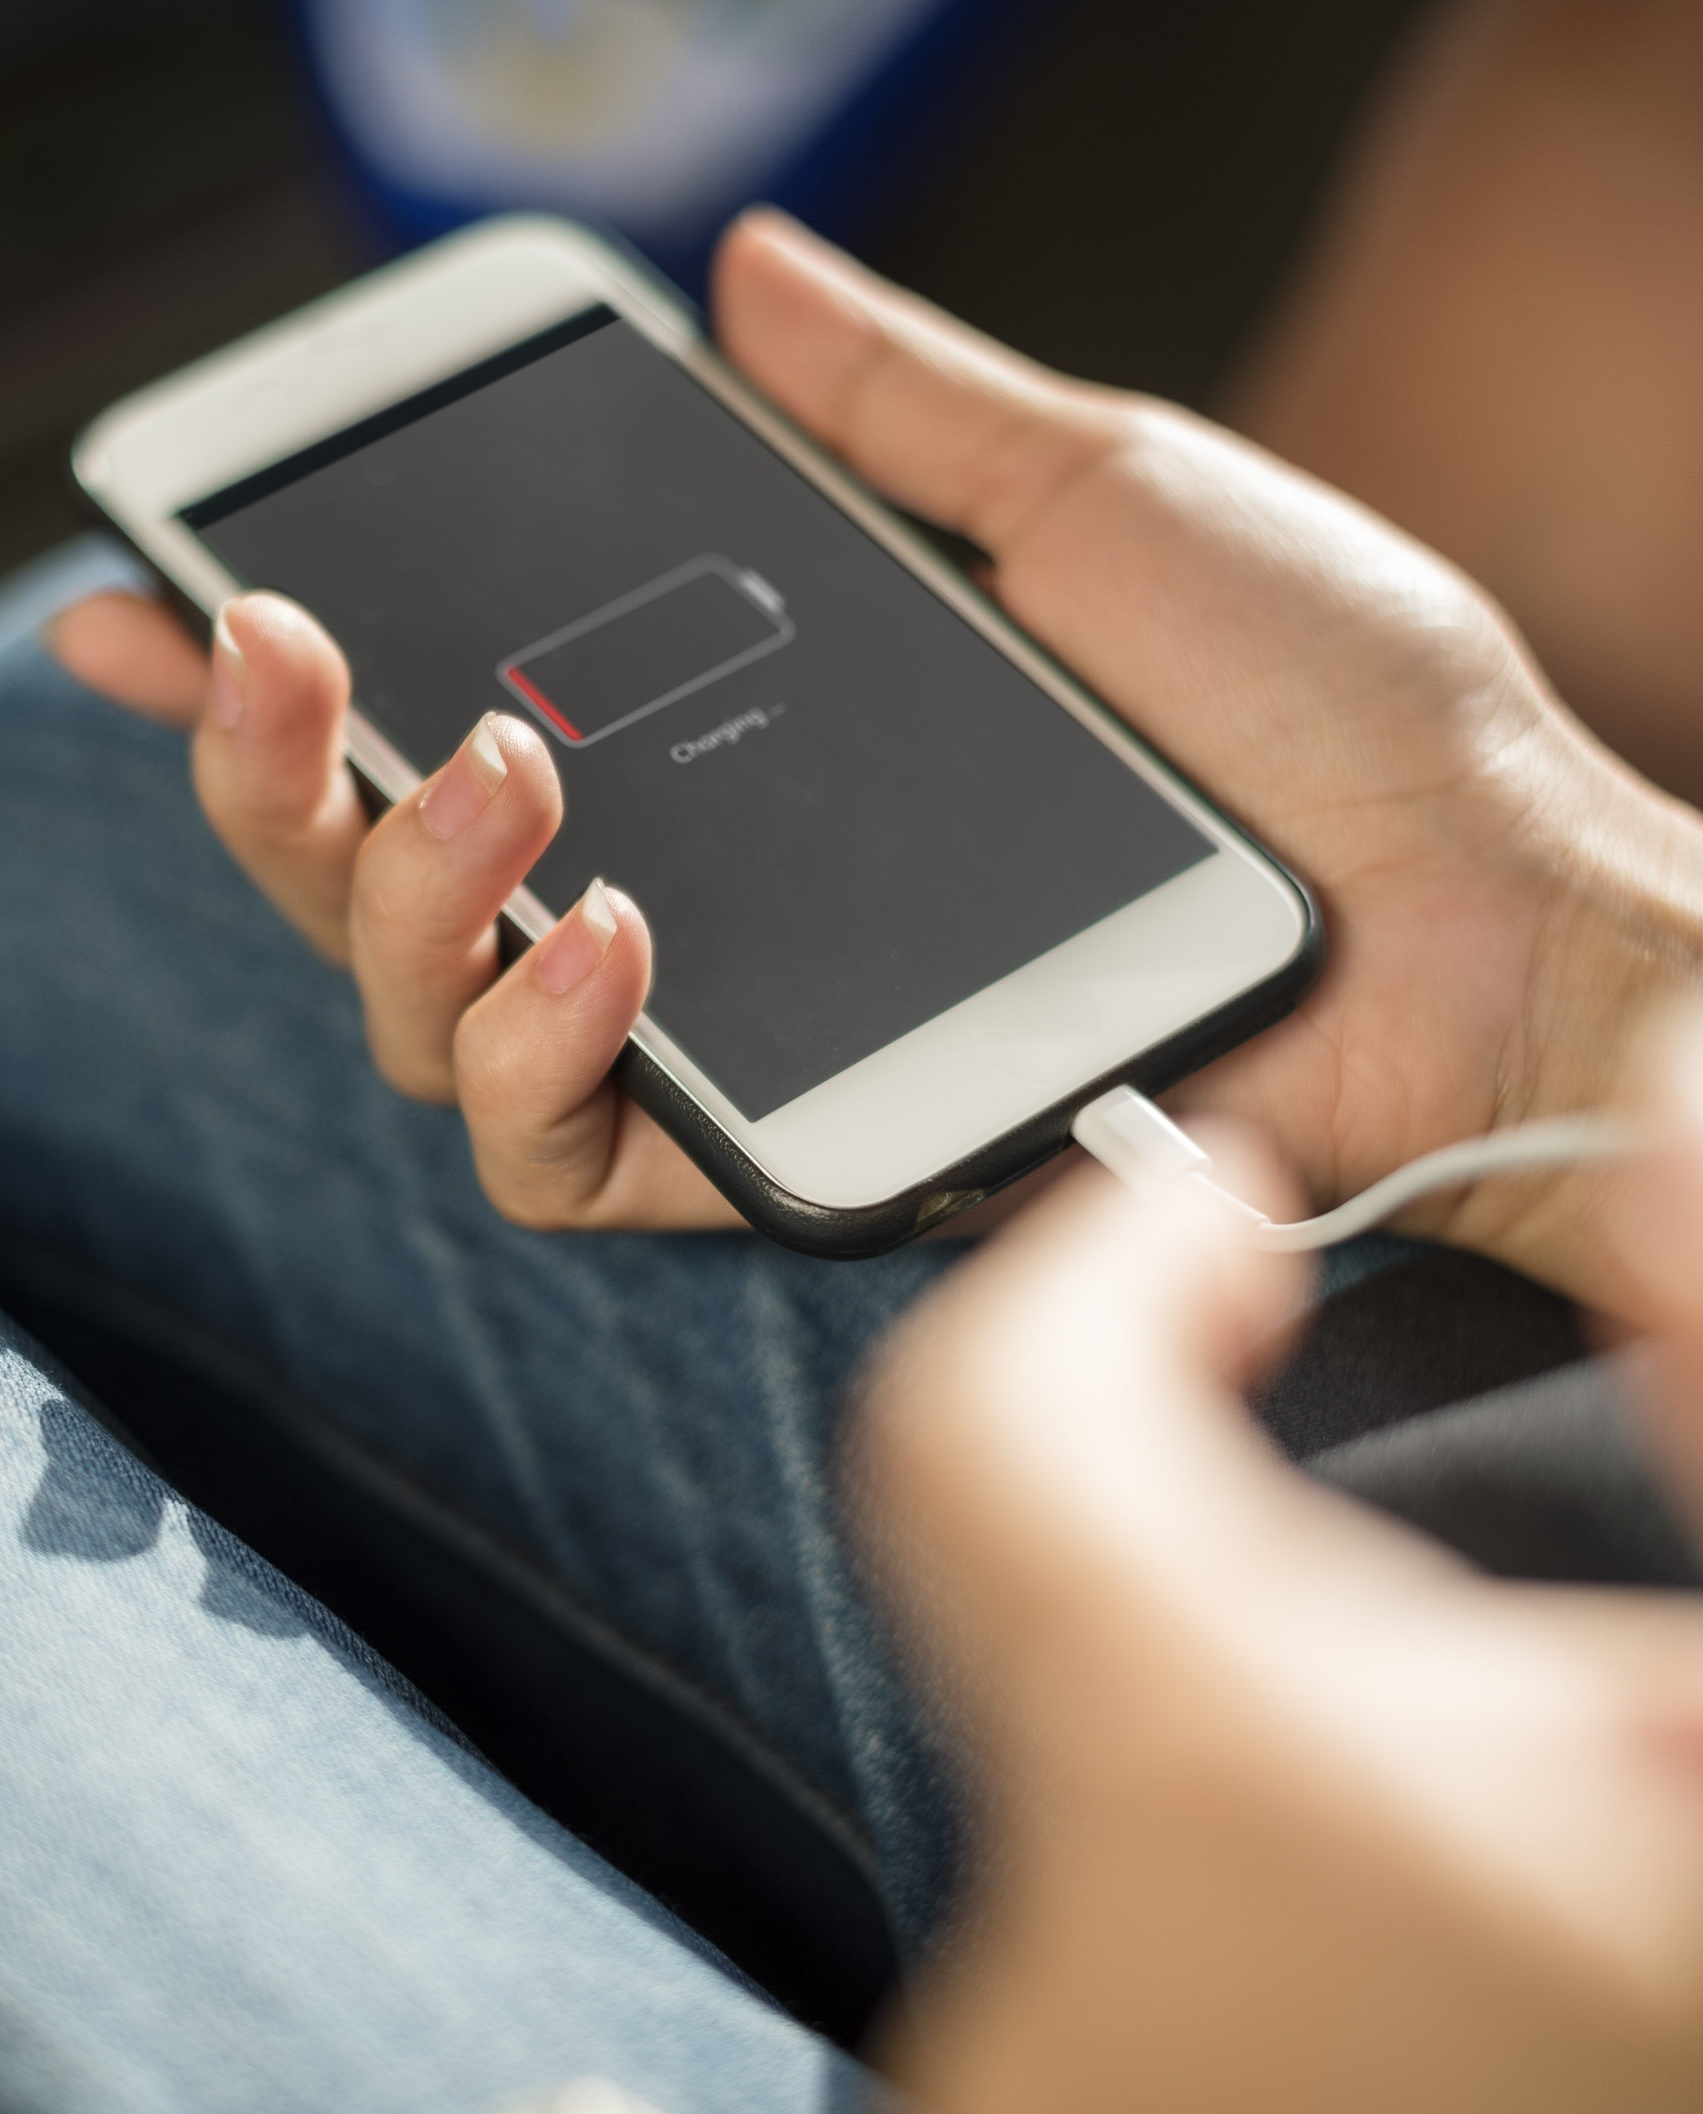
\includegraphics[width=4cm, height=4cm]{Figs/low_power.png}
			\caption*{Low Power}
		\end{minipage}
		\begin{minipage}[t]{0.4\textwidth}
			\centering
			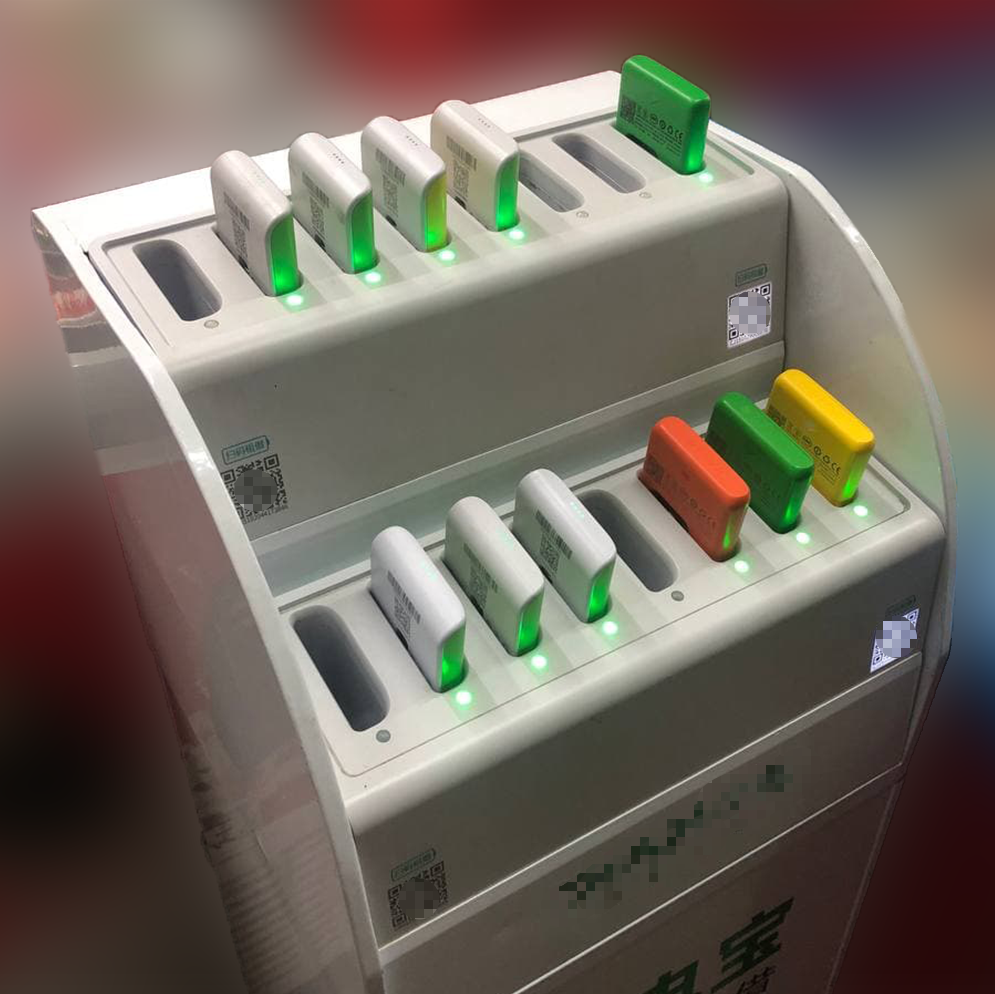
\includegraphics[width=4cm, height=4cm]{Figs/PBS_xd.png}
			\caption*{Sharing Powerbank}
		\end{minipage}
	\end{figure}
\end{frame}
\subsection{Procedure}
\begin{frame}{Typical Attack Procedure}
	\begin{enumerate}
		\item The attacker rents a power bank and replaces the internal components with BadUSB-C.
		\item An attacker-crafted power bank is returned to the rental station in crowded areas.
		\item A user borrows the modified power bank and connects it to his/her own device.
		\item The attacker can now fully control the victim's device.
	\end{enumerate}
\end{frame}
\subsection{Experiment}
\begin{frame}{Experiment Setup}
	We conducted experiment on a HUAWEI P30 Android smartphone. Eleven applications were selected and tested in the following steps:
	\begin{enumerate}
		\item Login in with a test account.
		\item Keep the default settings.
		\item Attach BadUSB-C to the test device.
		\item Simulate victim's daily usage of the application.
	\end{enumerate}
\end{frame}
\begin{frame}{Experiment Screenshots}
	\begin{figure}[htbp]
		\centering
		\begin{minipage}[t]{0.3\textwidth}
			\centering
			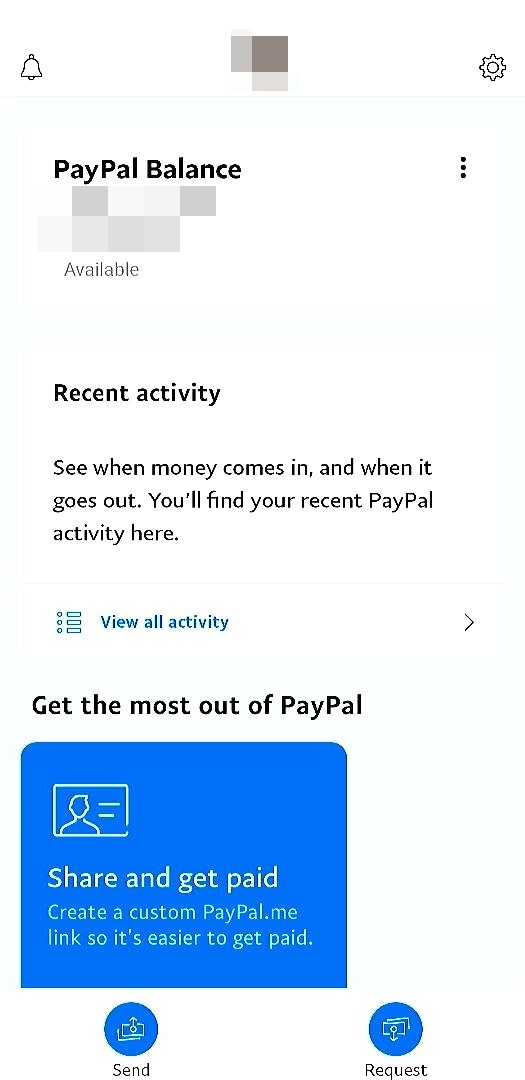
\includegraphics[width=\textwidth]{Figs/paypal.png}
		\end{minipage}
		\begin{minipage}[t]{0.3\textwidth}
			\centering
			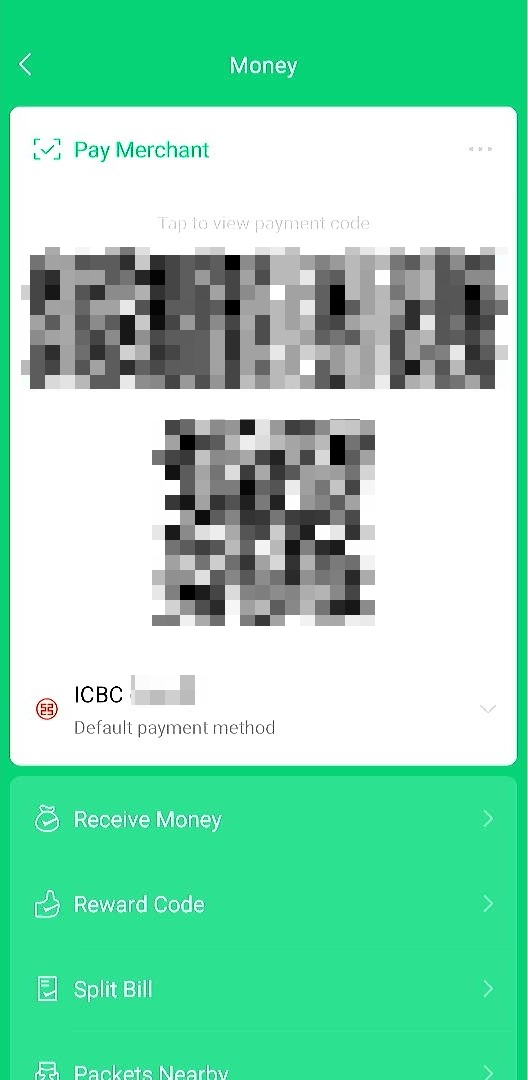
\includegraphics[width=\textwidth]{Figs/wechat.png}
		\end{minipage}
		\begin{minipage}[t]{0.3\textwidth}
			\centering
			
\includegraphics[width=\textwidth]{Figs/twitter.png}
		\end{minipage}
	\end{figure}
\end{frame}
\begin{frame}{Experiment Result}
	\begin{table}[htbp]
		\begin{tabular}{|l|l}
			\textbf{Application}         & \textbf{Leaked Sensitive Information} 		     \\
			WeChat      		         & Financial Status, History, Payment QR Code        \\
			WhatsApp                     & Contacts, Chat History, Phone Number              \\
			Alipay          			 & Financial Status, Payment QR Code                 \\
			Paypal 						 & Paypal Balance      							     \\                              
			Health                       & Personal Health Metrics                           \\
			...                          & ...                                               \\
		\end{tabular}
	\end{table}
\end{frame}
\section{Limitations}
\begin{frame}{Limitations}
	BadUSB-C also has serveral limitations.
	\begin{itemize}
		\item Cannot bypass biometrics authentications like fingerprint.
		\item Requires the DisplayPort over USB Type-C feature to work.
		\item May incur notifications on victim's devices and be discovered.
	\end{itemize}
\end{frame}
\section{Mitigation \& Responsible Disclosure}
\subsection{Mitigation}
\begin{frame}{Isolated UI Rendering}
	\begin{figure}
		\centering
		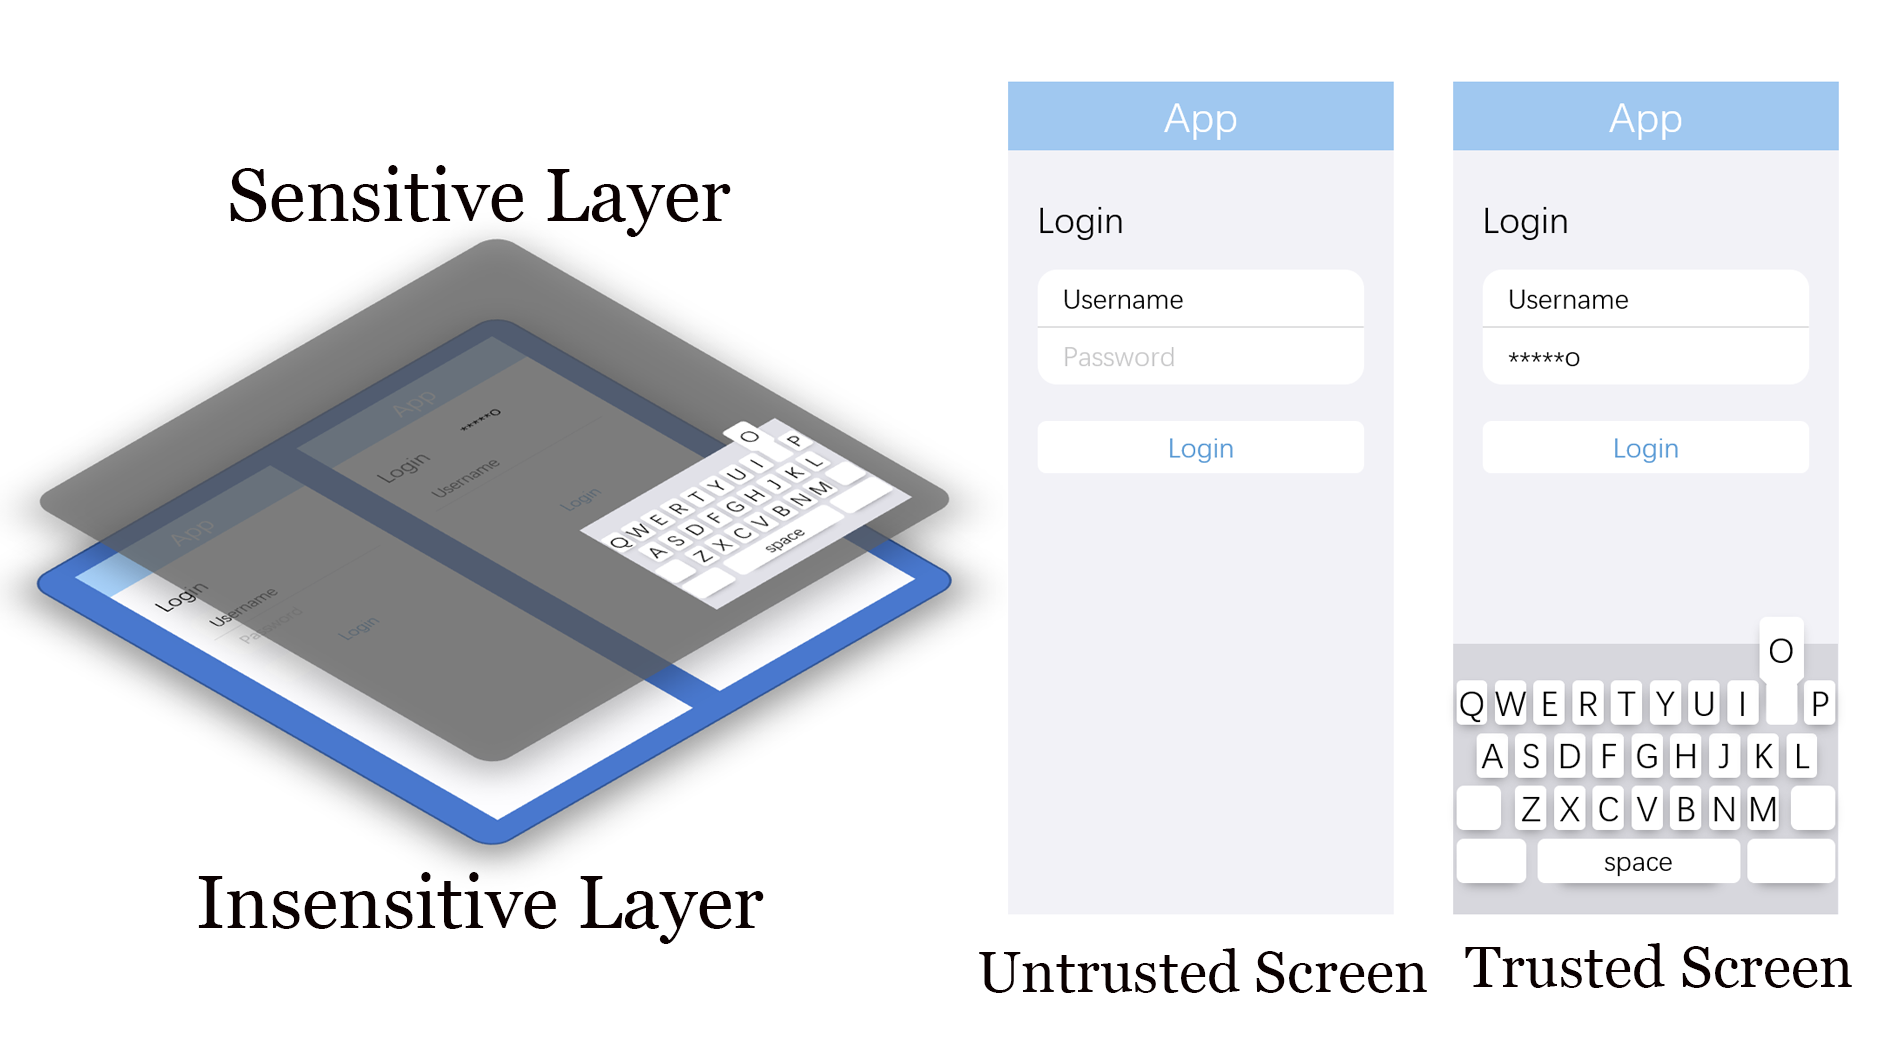
\includegraphics[width=\linewidth]{Figs/isolated_ui.png}
		\caption*{Isolated UI Rendering}
	\end{figure}
\end{frame}
\subsection{Responsible Disclosure}
\begin{frame}{Responsible Disclosure}
	We contacted HUAWEI after we discovered this vulnerability, who later assigned a CVE entry (CVE-2021-22325) for this vulnerability. 
	\begin{figure}
		\centering
		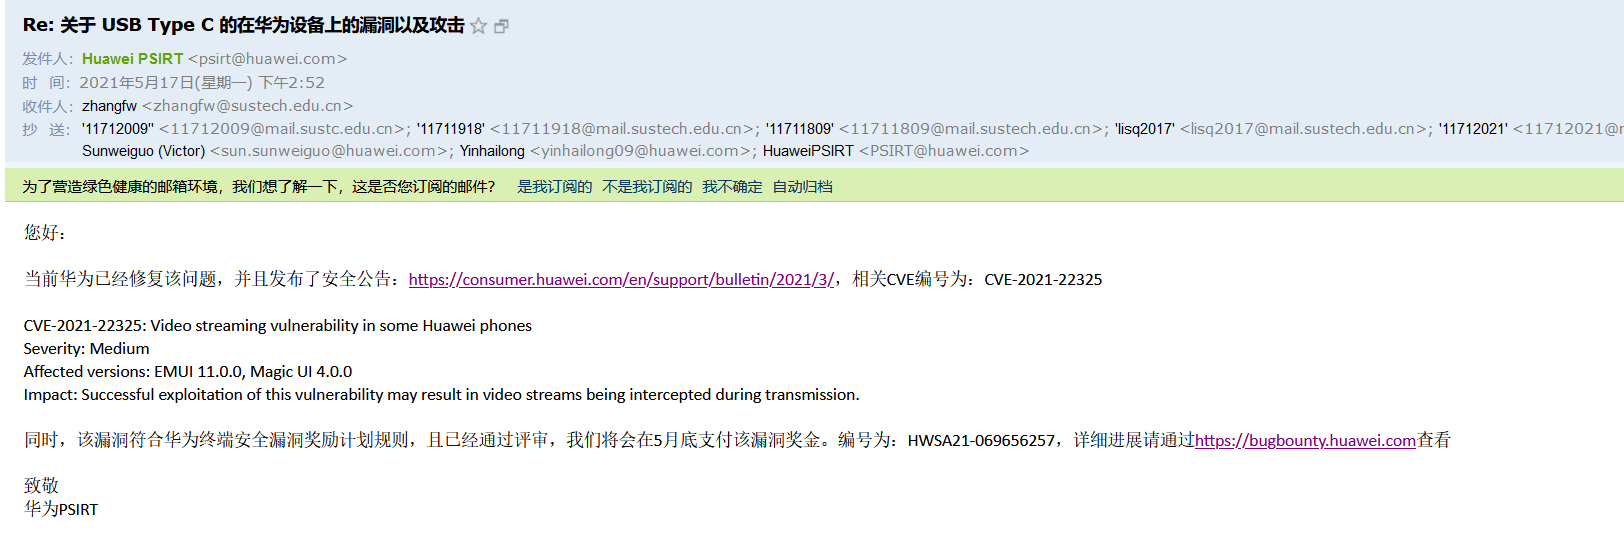
\includegraphics[width=\linewidth]{Figs/huawei_response.png}
		\caption*{HUAWEI Response}
	\end{figure}
\end{frame}
\begin{frame}{HUAWEI Bug Bounty}
We also applied for the bug bounty program of HUAWEI and gained a reward of over \$4500.
	\begin{figure}
		\centering
		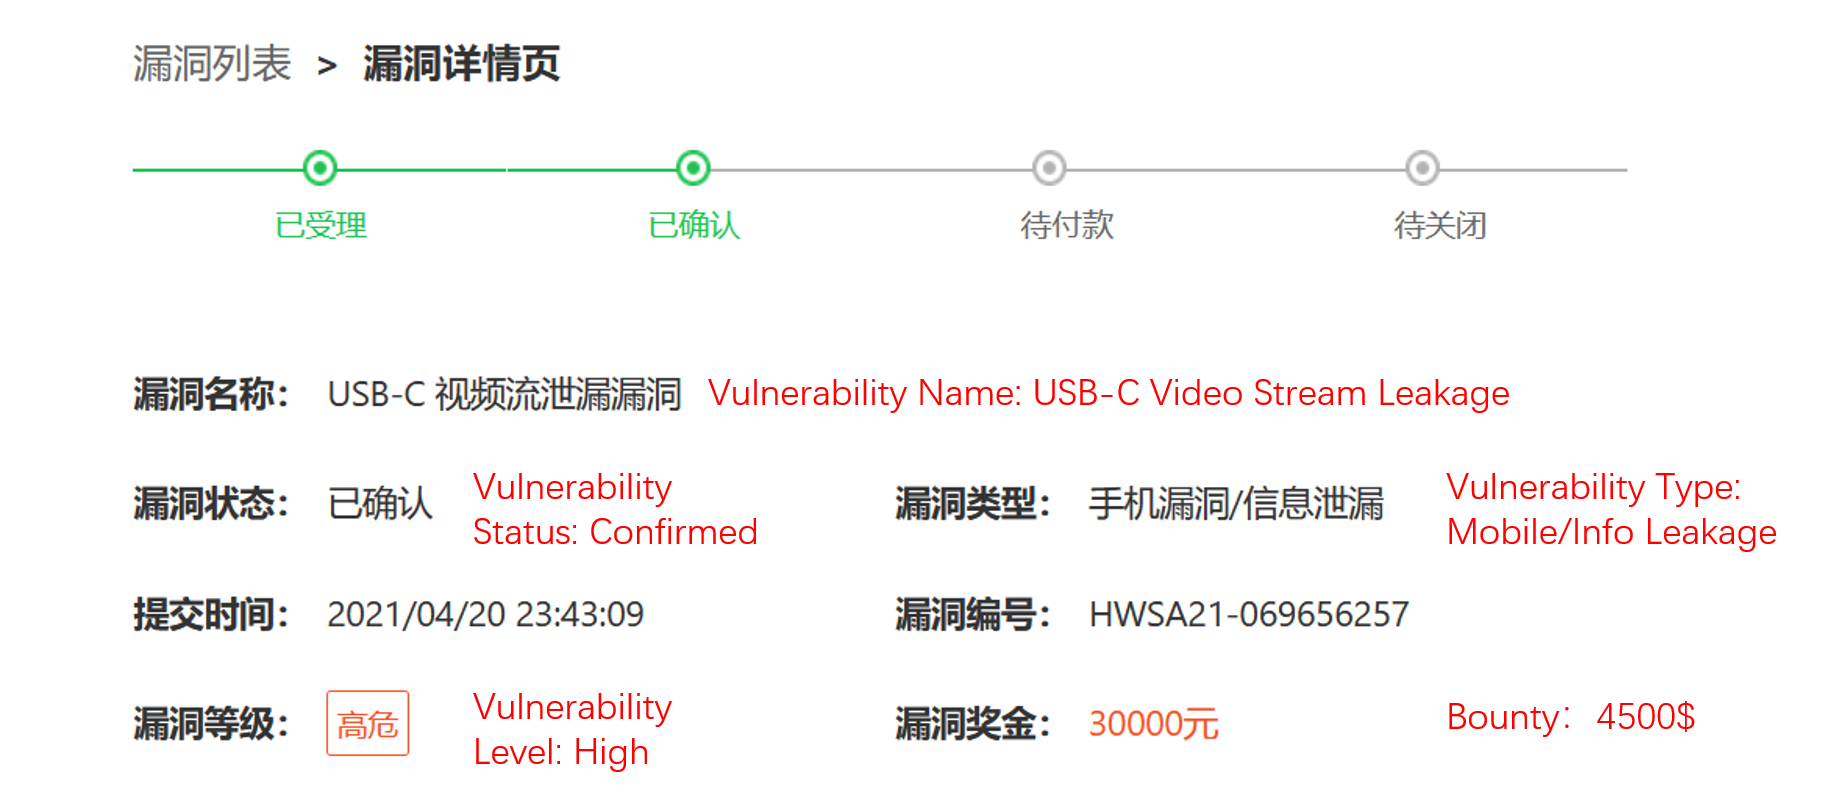
\includegraphics[width=\linewidth]{Figs/bounty.png}
		\caption*{HUAWEI Bug Bounty}
	\end{figure}
\end{frame}
\begin{frame}{Current Mitigation}
	\begin{columns}
		\column{.65\linewidth}
			Now, mitigation for this vulnerability has already been deployed.
			\vspace{1em}

			This mitigation requires user authentication before allowing external USB devices.
		\column{.35\linewidth}
			\begin{figure}
				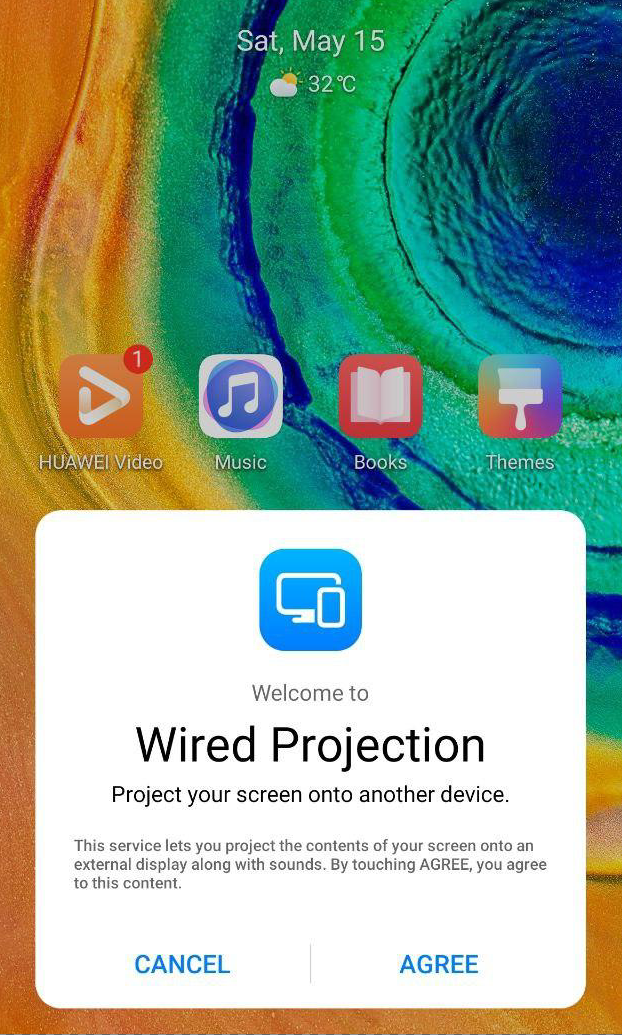
\includegraphics[width=\columnwidth]{Figs/huawei.png}
			\end{figure}
	\end{columns}
\end{frame}
\section{Conclusion}
\begin{frame}{Conclusion}
	We summarize our work as follows.
	\begin{enumerate}
		\item We explore a new attack scheme leveraging the latest feature of USB protocol.
		\item We conduct real-life scenario study of sharing powerbank to test BadUSB-C efficiency.
		\item We propose novel mitigation for our BadUSB-C attack.
	\end{enumerate}
\end{frame}
\begin{frame}
	\vfill
	\begin{center}
		\Large
		\emph{Thank You!}
	\end{center}
	\vfill
	\usebeamerfont{institute} \url{{11712009,11711918,lisq2017,11711809,11712021}@mail.sustech.edu.cn}
		\\ \url{zhangfw@sustech.edu.cn}
\end{frame}

\begin{frame}[allowframebreaks]
	\bibliographystyle{IEEEtran}
	\bibliography{ref.bib}
\end{frame}
\end{document}
